\section{Experiments}
\label{sec:experiments}
\subsection{Experimental Setup}
\label{sec:setup}

\paragraph{Models, datasets, and splits.}
We evaluate SIEVE on Qwen2.5-VL-7B \cite{Qwen2VL}, InternVL3-8B \cite{chen2024internvl}, and LLaVA-1.5-7B \cite{liu2023visual} using EarthVQA \cite{wang2024earthvqa}, LingoQA \cite{marcu2024lingoqa}, and VQAv2 \cite{balanced_vqa_v2}, yielding nine model--dataset tasks. Each task targets 5{,}000 fault-free executions and 50{,}000 random dual-bit fault injections; valid-execution counts are reported in Table~\ref{tab:A1} (appendix). Executions sharing the same image or question are assigned as a whole to disjoint Training / Validation / Test partitions (70\% / 15\% / 15\%). Faulty Training records train the Detector; fault-free telemetry within Training is further split into predictor fit / early-stopping / evaluation subsets under the same group rule. Validation freezes thresholds; Test is used only for final scoring.

\paragraph{Fault injection.}
We emulate transient soft errors by software fault injection: during prefill, we randomly select a \texttt{torch.nn.Linear} module and flip two random bits of a random scalar in its output tensor. Only executions that complete normally and yield extractable features are counted. Each faulty output is labeled Non-SDC, Non-significant SDC, or Significant SDC by an LLM judge, from its semantic change relative to the fault-free baseline on the same input.

\subsection{SDC Detector Evaluation}

\subsubsection{Detection Performance}
We perform nested selection over 40 feature-dimension/window combinations within the outer Training set only, ultimately adopting 36D with $K=28$: monitored pairs $(6,7)$, $(24,25)$, and $(26,27)$, aggregated over the first $\min(28,T)$ actual decoding steps (Appendix~\ref{app:config}). Neither Ranger nor Dr.DNA provides a public implementation, so we re-implement their detection mechanisms following the original papers to ensure a fair comparison under identical configurations, rather than claiming to reproduce the complete original systems. Concretely, all three methods share the same monitored layers, decoding steps, fault instances, and outer data partitions, and each freezes its threshold on the Validation set only; clean reference profiles for Ranger and Dr.DNA are built from a 20\% group subset determined in the Training set, with remaining details in Table~\ref{tab:A2}. During evaluation, all methods are scored on exactly the same executions, matched row-by-row by sample identity, output, and fault metadata, with effective coverage in Table~\ref{tab:A1}. Each task's XGBoost Detector is trained on the Training set, and its threshold is chosen on the Validation set to maximize Significant-SDC F1. As shown in Table~\ref{tab:det_no_filter}, on the Test set SIEVE improves the nine-task average F1 over Ranger and Dr.DNA by 10.33 and 11.38 percentage points.
\begin{table}[!ht]
  \centering
  \caption{Per-task Significant-SDC detection results on the Test set (\%); P/R/F1 denote Precision/Recall/F1.}
  \label{tab:det_no_filter}
  \footnotesize
  \setlength{\tabcolsep}{4pt}
  \renewcommand{\arraystretch}{1.05}
  \resizebox{\linewidth}{!}{%
  \begin{tabular}{llccccccccc}
  \toprule
  & & \multicolumn{3}{c}{\textbf{EarthVQA}} & \multicolumn{3}{c}{\textbf{LingoQA}} & \multicolumn{3}{c}{\textbf{VQAv2}} \\
  \cmidrule(lr){3-5} \cmidrule(lr){6-8} \cmidrule(lr){9-11}
  \textbf{Model} & \textbf{Method} & \textbf{P} & \textbf{R} & \textbf{F1} & \textbf{P} & \textbf{R} & \textbf{F1} & \textbf{P} & \textbf{R} & \textbf{F1} \\
  \midrule
  \multirow{3}{*}{Qwen2.5-VL-7B}
   & Ranger & 94.85  & 81.85 & 87.87 & 49.87  & 92.92 & 64.91 & 63.02  & 81.61 & 71.12 \\
   & Dr.DNA & 100.00 & 61.48 & 76.15 & 52.33  & 74.06 & 61.33 & 79.71  & 63.22 & 70.51 \\
   & SIEVE  & 89.54  & 85.56 & 87.50 & 99.49  & 92.93 & 96.10 & 100.00 & 84.29 & 91.48 \\
  \cmidrule(lr){2-11}
  \multirow{3}{*}{InternVL3-8B}
   & Ranger & 85.77  & 95.76 & 90.49 & 66.22  & 89.54 & 76.13 & 94.57  & 72.76 & 82.25 \\
   & Dr.DNA & 97.63  & 78.39 & 86.96 & 99.43  & 70.02 & 82.17 & 99.12  & 67.00 & 79.95 \\
   & SIEVE  & 99.57  & 97.67 & 98.61 & 99.35  & 91.75 & 95.40 & 97.06  & 91.85 & 94.38 \\
  \cmidrule(lr){2-11}
  \multirow{3}{*}{LLaVA-1.5-7B}
   & Ranger & 86.67  & 95.97 & 91.08 & 100.00 & 85.03 & 91.91 & 100.00 & 91.12 & 95.36 \\
   & Dr.DNA & 100.00 & 95.97 & 97.95 & 100.00 & 85.56 & 92.22 & 100.00 & 89.35 & 94.38 \\
   & SIEVE  & 95.36  & 96.64 & 96.00 & 99.41  & 90.37 & 94.68 & 87.64  & 92.31 & 89.91 \\
  \midrule
  \multirow{3}{*}{Average}
   & Ranger & 89.10 & 91.19 & 89.81 & 72.03 & 89.16 & 77.65 & 85.86 & 81.83 & 82.91 \\
   & Dr.DNA & 99.21 & 78.61 & 87.02 & 83.92 & 76.55 & 78.57 & 92.94 & 73.19 & 81.61 \\
   & \textbf{SIEVE} & \textbf{94.82} & \textbf{93.29} & \textbf{94.04} & \textbf{99.42} & \textbf{91.68} & \textbf{95.39} & \textbf{94.90} & \textbf{89.48} & \textbf{91.92} \\
  \bottomrule
  \end{tabular}%
  }
\end{table}

Some executions produce NaN or $\pm\mathrm{Inf}$ values among the monitored features after injection, and such extreme values are trivially detected by any method. To verify whether the methods genuinely distinguish the harder cases, we filter out these executions and re-score all three methods on the remaining ones whose 36 features are all finite, with no retraining or recalibration; Table~\ref{tab:det_finite} reports the result. The average F1 of Ranger and Dr.DNA drops from 83.46 and 82.40 in Table~\ref{tab:det_no_filter} to 37.74 and 22.74, whereas SIEVE degrades far less (93.78 to 68.78) and exceeds both baselines by a wide margin on most tasks, attaining the highest F1 on seven of the nine. Its advantage therefore comes from discriminating genuinely ambiguous finite-value faults rather than from obvious non-finite signals.

\begin{table}[!ht]
  \centering
  \caption{Per-task Significant-SDC detection on the Test set after excluding executions with non-finite features (\%).}
  \label{tab:det_finite}
  \footnotesize
  \setlength{\tabcolsep}{4pt}
  \renewcommand{\arraystretch}{1.05}
  \resizebox{\linewidth}{!}{%
  \begin{tabular}{llccccccccc}
  \toprule
  & & \multicolumn{3}{c}{\textbf{EarthVQA}} & \multicolumn{3}{c}{\textbf{LingoQA}} & \multicolumn{3}{c}{\textbf{VQAv2}} \\
  \cmidrule(lr){3-5} \cmidrule(lr){6-8} \cmidrule(lr){9-11}
  \textbf{Model} & \textbf{Method} & \textbf{P} & \textbf{R} & \textbf{F1} & \textbf{P} & \textbf{R} & \textbf{F1} & \textbf{P} & \textbf{R} & \textbf{F1} \\
  \midrule
  \multirow{3}{*}{Qwen2.5-VL-7B}
   & Ranger & 83.78  & 55.86 & 67.03 & 20.80  & 77.61 & 32.81 & 27.75  & 50.00 & 35.69 \\
   & Dr.DNA & 100.00 & 18.92 & 31.82 & 11.18  & 26.87 & 15.79 & 8.70   & 4.17  & 5.63 \\
   & SIEVE  & 72.73  & 64.86 & 68.57 & 98.11  & 77.61 & 86.67 & 100.00 & 57.29 & 72.85 \\
  \cmidrule(lr){2-11}
  \multirow{3}{*}{InternVL3-8B}
   & Ranger & 58.56  & 84.13 & 69.06 & 30.37  & 65.56 & 41.51 & 60.38  & 18.93 & 28.83 \\
   & Dr.DNA & 79.07  & 26.98 & 40.24 & 85.71  & 7.95  & 14.55 & 80.00  & 7.10  & 13.04 \\
   & SIEVE  & 98.29  & 91.27 & 94.65 & 97.35  & 72.85 & 83.33 & 90.14  & 75.74 & 82.32 \\
  \cmidrule(lr){2-11}
  \multirow{3}{*}{LLaVA-1.5-7B}
   & Ranger & 21.43  & 50.00 & 30.00 & 0.00   & 0.00  & 0.00  & 100.00 & 21.05 & 34.78 \\
   & Dr.DNA & 100.00 & 50.00 & 66.67 & 100.00 & 3.57  & 6.90  & 100.00 & 5.26  & 10.00 \\
   & SIEVE  & 50.00  & 58.33 & 53.85 & 90.91  & 35.71 & 51.28 & 21.43  & 31.58 & 25.53 \\
  \midrule
  \multirow{3}{*}{Average}
   & Ranger & 54.59 & 63.33 & 55.36 & 17.06 & 47.72 & 24.77 & 62.71 & 29.99 & 33.10 \\
   & Dr.DNA & 93.02 & 31.97 & 46.24 & 65.63 & 12.80 & 12.41 & 62.90 & 5.51  & 9.56 \\
   & \textbf{SIEVE} & \textbf{73.67} & \textbf{71.49} & \textbf{72.36} & \textbf{95.46} & \textbf{62.06} & \textbf{73.76} & \textbf{70.52} & \textbf{54.87} & \textbf{60.23} \\
  \bottomrule
  \end{tabular}%
  }
\end{table}

\subsubsection{Detection Overhead}
\begin{wraptable}{l}{3.1in}
  \vspace{-12pt}
  \refstepcounter{table}%
  {\raggedright Table~\thetable: End-to-end mean latency and relative overhead (\%) on LingoQA.\par}
  \label{tab:sieve_online_overhead}
  \vspace{2pt}
  \small
  \resizebox{2.95in}{!}{%
  \begin{tabular}{lcccc}
    \toprule
    Model & Baseline & Ranger & Dr.DNA & SIEVE \\
    \midrule
    Qwen2.5-VL-7B   & 764.4 & +1.77 & +3.82 & +6.44 \\
    InternVL3-8B    & 984.3 & +1.78 & +5.20 & +6.53 \\
    LLaVA-1.5-7B    & 363.8 & +2.75 & +5.67 & +6.98 \\
    \bottomrule
  \end{tabular}%
  }
\end{wraptable}
We measure end-to-end overhead on a single NVIDIA H20 GPU with batch size 1. All four detection modes use the same six monitored layers and run over the first $\min(28,T)$ actual decoding steps. Each model executes 10 warmup and 10 forward repetitions on 50 fixed LingoQA samples, yielding 500 observations per model--method pair. Answers under all monitored modes are identical to the baseline without detection. SIEVE's average overhead is 6.65\%, versus 2.10\% for Ranger and 4.89\% for Dr.DNA.

\subsection{Nominal Inter-Layer Predictor Evaluation}
As shown in Table~\ref{tab:fault_free_predictor_performance} (appendix), the trained Nominal Inter-Layer Predictor attains MSE from 0.0066 to 0.2207 and CosSim from 0.6367 to 0.9138 across the nine tasks; because activation scales differ across models, MSE is not comparable across models. We further examine how the prediction residual behaves under faults. Figure~\ref{fig:cosine-vis} shows the CosSim averaged over all actual decoding steps for each faulty run: Significant SDCs exhibit the lowest mean CosSim, while Non-SDC and Non-significant SDC overlap clearly, confirming that the predictor separates Significant SDCs from Non-significant SDCs well.

\begin{figure}[!ht]
\centering
    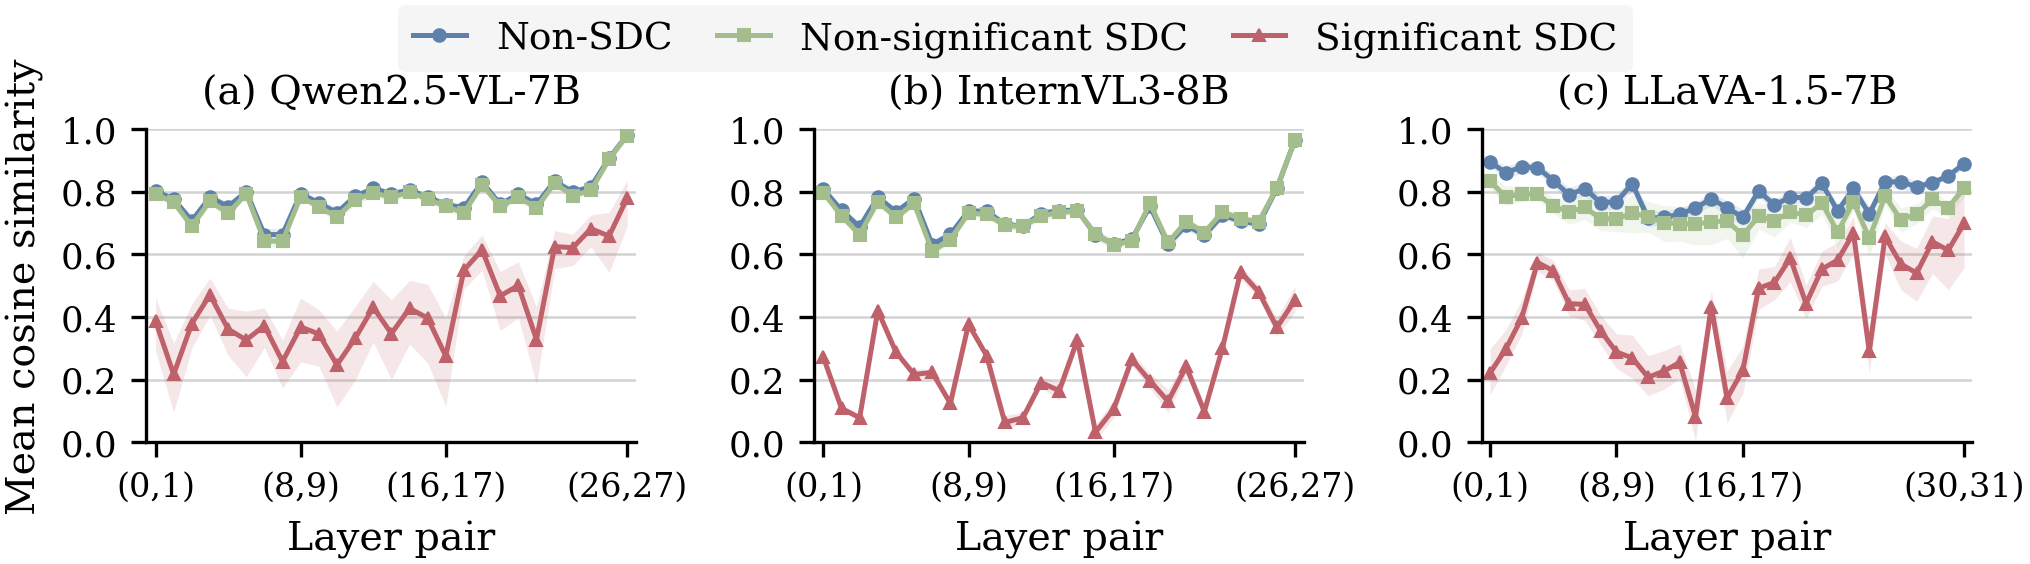
\includegraphics[width=1.0\linewidth]{Figures/figure6_layer_pair_cosine_similarity.png}
    \caption{Average finite CosSim per adjacent layer pair over actual decoding steps on LingoQA, grouped by execution category. Shaded bands are 95\% cluster bootstrap confidence intervals over images.}
    \label{fig:cosine-vis}
\end{figure}

\subsection{Ablation Study}
We ablate layer pairs and metrics at the fixed 36D/K=28 configuration. Layer-pair ablation removes all 12 features of one pair; metric ablation removes the 9 features of CosSim, Mean Difference, Std Difference, or L2 Distance across the three pairs. We additionally score only the executions whose 36 features are all finite, after the configuration has been frozen. As Figure~\ref{fig:ablation} shows, removing any component lowers the nine-task average Test F1. Removing $(26,27)$ and $(24,25)$ costs 2.47 and 2.16 F1 points, respectively; among metrics, Mean Difference is most critical ($-3.74$) and Std Difference contributes least ($-0.46$). The finite-value diagnostic shows the same overall trend. Complete per-task results on the Test set are in Table~\ref{tab:A5}, and those of the finite-value diagnostic are in Table~\ref{tab:A6} (appendix).

\begin{figure}[!ht]
\centering
    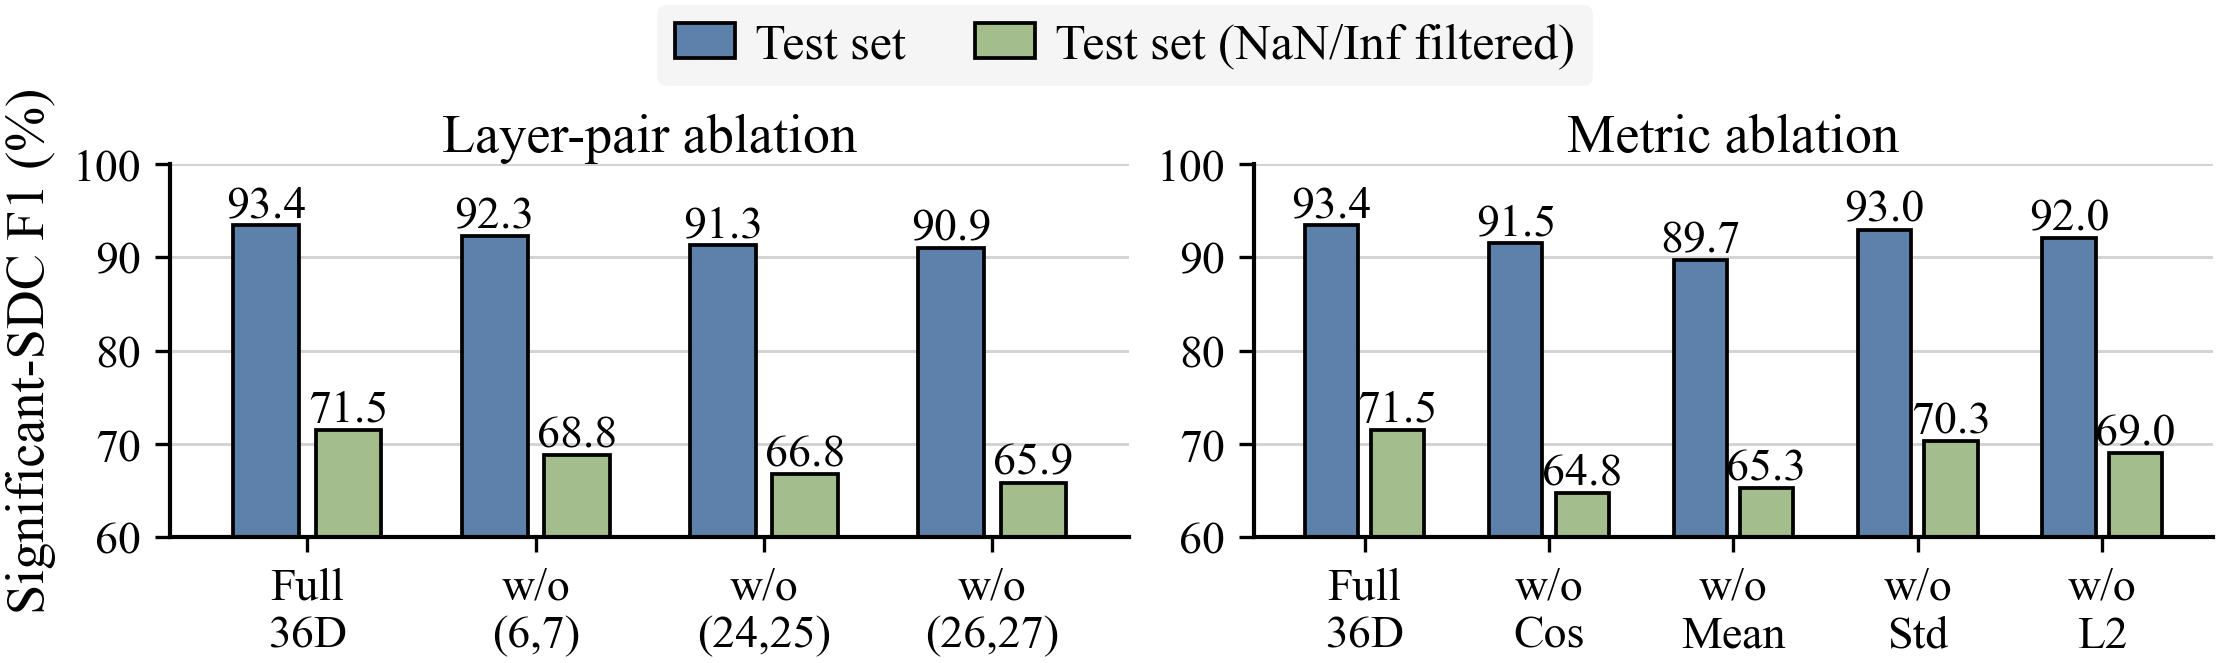
\includegraphics[width=1.0\linewidth]{Figures/figure7_component_ablation.png}
    \caption{Component ablation at 36D/K=28. Left: layer-pair ablation; right: metric ablation. Bars show nine-task average Significant-SDC F1.}
    \label{fig:ablation}
\end{figure}


